\section{$\lambdaLVar$: Syntax and Semantics}\label{s:lvars-lambdalvar}

\lk{Figures~\ref{f:lvars-lambdaLVar-syntax} and
  \ref{f:lvars-lambdaLVar-semantics} are a first stab at cutting the
  handlers/quiescence/freezing stuff out of the POPL formalism.  Needs
  to be looked at more closely.}

\FigLambdaLVarGrammar

\FigLambdaLVarSemantics

The syntax and operational semantics of $\lambdaLVar$ appear in
Figures~\ref{f:lvars-lambdaLVar-syntax} and
\ref{f:lvars-lambdaLVar-semantics}, respectively.\footnote{We have
  implemented $\lambdaLVar$ as a runnable PLT Redex \cite{redex-book}
  model, available in the LVars repository.}  As we have noted, both
the syntax and semantics are parameterized by the lattice $D$.  The
reduction relation $\parstepsto$ is defined on \emph{configurations}
$\config{S}{e}$ comprising a store and an expression.  The \emph{error
  configuration}, written $\error$, is a unique element added to the
set of configurations, but we consider $\config{\topS}{e}$ to be equal
to $\error$, for all expressions $e$.  The metavariable $\conf$ ranges
over configurations.

\TODO{Explain the rules in Figure~\ref{f:lvars-lambdaLVar-semantics}
  using either text from my thesis proposal or the POPL paper (leaving
  out the handlers/quiescence/freezing stuff.}

\subsection{Fork-Join Parallelism}\label{subsection:fork-join}

$\lambdaLVar$ has a call-by-value semantics: arguments must be fully
evaluated before function application ($\beta$-reduction, modeled by
the {\sc E-Beta} rule) can occur.  We can exploit this property to
define a syntactic sugar $\LETPAR$ for \emph{parallel composition},
which computes two subexpressions $e_1$ and $e_2$ in parallel before
computing $e_3$:
\begin{displaymath}
\begin{minipage}[b]{0.8in}
  \begin{equation*}
\begin{split}
& \LETPAR ~x = e_1 \\ 
& \letparspace ~y = e_2 \\
& \letspace \IN~e_3 
\end{split}
\end{equation*}
\end{minipage}
\begin{minipage}[b]{0.6in}
\centering
$\defeq$
\end{minipage}
\begin{minipage}[b]{1in}
\begin{equation*}
  \app{(\app{(\lam{x}{(\lam{y}{e_3})})}{e_1})}{e_2}
\end{equation*}
\end{minipage}
\end{displaymath}
\noindent Although $e_1$ and $e_2$ can be evaluated in parallel, $e_3$
cannot be evaluated until both $e_1$ and $e_2$ are values, because the
call-by-value semantics does not allow $\beta$-reduction until the
operand is fully evaluated, and because it further disallows reduction
under $\lambda$-terms (sometimes called ``full $\beta$-reduction'').
In the terminology of parallel programming, a $\LETPAR$ expression
executes both a \emph{fork} and a \emph{join}.  Indeed, it is common for
fork and join to be combined in a single language construct, for
example, in languages with parallel tuple expressions such as
Manticore~\cite{manticore_parallel_tuples}.

\begin{figure}[tb]
  \centering 
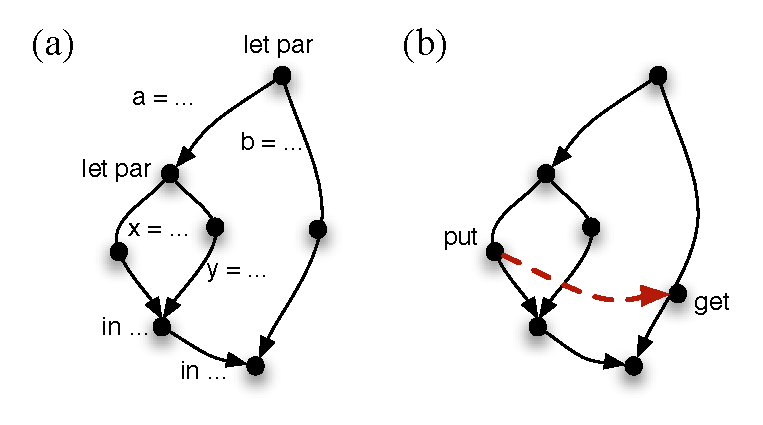
\includegraphics[width=4in]{chapter2/figures/SeriesParallel.pdf} 
\caption{\footnotesize A series-parallel graph induced by parallel
    $\lambda$-calculus evaluation (a); a non-series-parallel
    graph induced by $\PUT$/$\GET$ operations (b).}
  \label{f:series-parallel}
\end{figure}

Since $\LETPAR$ expresses \emph{fork-join} parallelism, the evaluation
of a program comprising nested $\LETPAR$ expressions would induce a
runtime dependence graph like that pictured in
Figure~\ref{f:series-parallel}(a).  The $\lambdaLVar$ language (minus
$\PUT$ and $\GET$) can support any \emph{series-parallel} dependence
graph.  Adding communication through $\PUT$ and $\GET$ introduces
``lateral'' edges between branches of a parallel computation, as in
Figure~\ref{f:series-parallel}(b).  This adds the ability to construct
arbitrary non-series-parallel dependency graphs, just as with
\emph{first-class futures}~\cite{beyond-nested-workstealing}.

Because we do not reduce under $\lambda$-terms, we can sequentially
compose $e_1$ before $e_2$ by writing $\letexp{\_}{e_1}{e_2}$, which
desugars to $\app{(\lam{\_}{e_2})}{e_1}$.  Sequential composition is
useful for, for instance, allocating a new LVar before beginning a
sequence of side-effecting $\PUT$ and $\GET$ operations on it.

\subsection{Programming with $\PUT$ and $\GET$}\label{subsection:programming-with-put-and-get}

For our first example of a $\lambdaLVar$ program, we choose the
elements of our lattice to be pairs of natural-number-valued IVars, as
shown in Figure~\ref{f:lattice-examples}(b).  We can then write the
following program:
\begin{equation}
\begin{split}
& \letexp{p}{\NEW}{ \\
& \letspace \letexp{\_}{\putexp{p}{\stateset{(3,4)}}}{ \\
& \letspace \letspace \letexp{v_1}{\getexp{p}{\stateset{(\bot, n) \setsep n \in \mathbb{N}}}}{ \\
& \letspace \letspace \letspace \dots v_1 \dots}}}
\end{split}
\label{e:getSnd}
\end{equation}
This program creates a new LVar $p$ and stores the pair $(3, 4)$ in
it.  $(3,4)$ then becomes the \emph{state} of $p$.  The premises of
the {\sc E-GetVal} reduction rule hold: $S(p) = (3,4)$; the threshold
set $Q = \stateset{(\bot, n) \setsep n \in \mathbb{N}}$ is a pairwise
incompatible subset of $D$; and there exists an element $d_1 \in Q$
such that $d_1 \userleq (3,4)$.  In particular, the pair $(\bot, 4)$
is a member of $Q$, and $(\bot,4) \userleq (3,4)$.  Therefore,
$\getexp{p}{\stateset{(\bot, n) \setsep n \in \mathbb{N}}}$ returns
the singleton set $\stateset{(\bot,4)}$, {which is a first-class value
  in $\lambdaLVar$ that can, for example, subsequently be passed to
  $\PUT$.}

Since threshold sets can be cumbersome to read, we can define some
convenient shorthands $\GETFST$ and $\GETSND$ for working with our
lattice of pairs:
\begin{align*}
\getfstexp{p} \defeq \getexp{p}{\stateset{(n, \bot) \setsep n \in
    \mathbb{N}}} \\
\getsndexp{p} \defeq \getexp{p}{\stateset{(\bot, n) \setsep n \in
    \mathbb{N}}}
\end{align*}
The approach we take here for pairs generalizes to arrays of arbitrary
size, with \emph{streams} being the special case of unbounded arrays
where consecutive locations are written.

\paragraph{Querying incomplete data structures}

It is worth noting that $\getsndexp{p}$ returns a value even if the
first entry of $p$ is not filled in.  For example, if the $\PUT$ in
the second line of \eqref{e:getSnd} had been
$\putexp{p}{\stateset{(\bot,4)}}$, the $\GET$ expression would still
return $\stateset{(\bot,4)}$.  It is therefore possible to safely
query an incomplete data structure---say, an object that is in the
process of being initialized by a constructor.  However, notice that
we {\em cannot} define a $\GETFSTORSND$ function that returns if
either entry of a pair is filled in.  Doing so would amount to passing
all of the boxed elements of the lattice in
Figure~\ref{f:lattice-examples}(b) to $\GET$ as a single threshold
set, which would fail to satisfiy the incompatibility criterion.

\paragraph{Blocking reads}

On the other hand, consider the following:
\begin{equation}
\begin{split}
& \letexp{p}{\NEW}{ \\
& \letspace \letexp{\_}{\putexp{p}{\stateset{(\bot,4)}}}{ \\
& \letspace \letspace \LETPAR ~v_1 = \getfstexp{p} \\
& \letspace \letspace \letparspace \hspace{0.62em}\_~= \putexp{p}{\stateset{(3,4)}} \\
& \letspace \letspace \letspace \IN~ \dots~v_1~\dots }}
\end{split}
\label{e:getSndWithBlock}
\end{equation}
Here $\GETFST$ can attempt to read from the first entry of $p$ before
it has been written to.  However, thanks to $\LETPAR$, the $\GETFST$
operation is being evaluated in parallel with a $\PUT$ operation that
will give it a value to read, so $\GETFST$ simply {\em blocks} until
$\putexp{p}{\stateset{(3,4)}}$ has been evaluated, at which point the
evaluation of $\getfstexp{p}$ can proceed.

In the operational semantics, this blocking behavior corresponds to
the last premise of the {\sc E-GetVal} rule not being satisfied.  In
\eqref{e:getSndWithBlock}, although the threshold set $\stateset{(n,
  \bot) \setsep n \in \mathbb{N}}$ is incompatible, the {\sc E-GetVal}
rule cannot apply because there is no state in the threshold set that
is lower than the state of $p$ in the lattice---that is, we are trying
to $\GET$ something that is not yet there!  It is only after $p$'s
state is updated that the premise is satisfied and the rule applies.
